
\begin{frame}[fragile]
    \frametitle{Инструменты правки топологии в GRASS}
    Основные инструменты:
    \begin{itemize}
        \item v.build --- построение топлогии (вызывается автоматически при импорте объектов);
        \item v.clean --- основной инструмент обработки топологии:
        \begin{verbatim}
        v.clean input=name output=name
        [type=string[,string,...]]
        [error=name]
        tool=string[,string,...]
        [thresh=float[,float,...]]
        \end{verbatim}
    \end{itemize}
\end{frame}

\begin{frame}[fragile]
    \frametitle{Основные параметры v.clean}
    \begin{verbatim}
    v.clean input=name output=name
    [type=string[,string,...]] [error=name]
    tool=string[,string,...] [thresh=float[,float,...]]
    \end{verbatim}
    \begin{itemize}
        \item input: название входной векторной карты, для которой проверяется/чистится топология
        \item output: название выходной векторной карты, в которой сохраняется результат
        \item type: тип объектов, которы обрабатываются (point, line, boundary, centroid, area, face, kernel). По умолчанию: point, line, boundary, centroid, area
        \item error: название выходной карты, в которую записываются ошибки
        \item tool: инструменты обработки
        \item thresh: пороговые значения для инструментов обработки топологии
    \end{itemize}
\end{frame}

\begin{frame}[allowframebreaks]
    \frametitle{Tool}
    \begin{itemize}
        \item break: Разбивать линии на пересечениях. Также разбивает линнии, если они образуют <<сплющеные>> петли. Например, линия (0 0, 1 0, 0 0) будет разбита на две: (0 0, 1 0) и (1 0, 0 0).
        \item snap: Притягивание вершин друг к другу в пределах заданного порога. При большом пороге может повреждать топологии при type=boundary. (Такие <<притянутые>> границы могут быть обработаны последовательностью break,rmdupl,rmsa).
        \item rmdangle: Удаление <<висящих>> узлов.
        \item chdangle: Изменение типа <<висящего>> узла с границы на линию.
        \item rmbridge: Удаление <<мостов>> между островами.
        \item chbridge: Изменение типа <<моста>> между островами с границы на линию.
        \item rmdupl: Удаляет дубликаты геометрий. (Категории!!!) Удобно использовать после инструмента break.
        \item rmdac: Удаляет дубликаты центроидов (они могут появляться после удаления границ).
        \item bpol: Чистит топологию при импорте из нетопологического формата. Границы разбиваются в каждой точке, общей для двух геометрий. (Похоже на break, но работает быстрее, зато требует больше памяти). После применения стоит прогнать rmdupl.
        \item prune: Прореживает узлы, которые лежат ближе указанного порога. Если чистятся границы, то топология сохраняется (отличие от snap).
        \item rmarea: Удаляет площади, которые меньше заданного порога. Удаление площади происходит за счет удаление наиболее протяженной общей границы и удаления всех неразделяемых границ.
        \item rmline: Удаление всех линий нулевой длины.
        \item rmsa: Удаление <<щелей>>:
        \begin{figure}[!ht]
            \begin{center}
                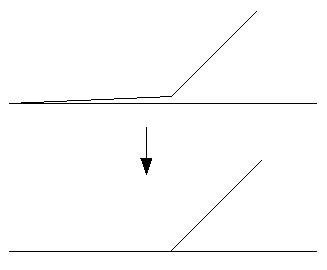
\includegraphics[width=0.4\columnwidth]{./grass/img/v_clean_rmsa}
            \end{center}
        \end{figure}
    \end{itemize}
\end{frame}

\begin{frame}[fragile]
    \frametitle{Генерализация инструментами GRASS GIS}
    \begin{itemize}
        \item Генерализация в момент импорта данных (уделение полигонов меньших заданого порога, <<прищелкивание>> узлов):
\begin{verbatim}
v.in.ogr -e dsn=regions2010.shp out=regions
    min_area=1 snap=100
\end{verbatim}


        \item v.clean:
\begin{verbatim}
v.clean in=regions out=sipmle type=boundary
    tool=prune,rmarea thresh=2000,4000000
\end{verbatim}
        \item v.generalize: специальный инструмент генерализации:
\begin{verbatim}
v.generalize input=name output=name
[type=string[,string,...]]
method=string threshold=float
...
[where=sql_query]
\end{verbatim}
    \end{itemize}
\end{frame}

\begin{frame}[allowframebreaks]
    \frametitle{Обзор методов упрощения геометрий v.generalize}
    \begin{itemize}
        \item Инструмент reduction -- самый простой алгоритм из представленных, удаляет точки линии, которые лежат около друг-друга ближе, чем на заданное пороговое расстояние. Таким образом, алгоритм использует один задаваемый пользователем параметр -- максимально допустимое расстояние, при котором точки считаются идентичными.
        \item Инструмент douglas реализует классический алгоритм Дугласа-Пекера. Инструмент принимает один параметр -- максимальное допустимое отклонение генерализованной линии от изначальной.
        \item Инструмент douglas\_reduction представляет собой модификацию алгоритма Дугласа-Пекера, в которой задается дополнительный параметр -- желаемое количество точек генерализованной линии, которое требуется достичь (измеряется в процентах по сравнению с количеством точек исходной линии).
        \item Инструмент lang также похож на алгоритм Дугласа-Пекера. Основное отличие состоит в том, что lang представляет собой не рекурсивный алгоритм. Поэтому, во избежание рекурсии алгоритм использует дополнительный параметр (look\_ahead), задающий число точек, которые требуется просмотреть
        \item Инструмент reumann использует коридор из двух параллельных линий заданной ширины. Для построения коридора берутся две последовательные точки линии и в направлении, заданном отрезком между точками строится коридор. Далее определяется место выхода линии за границы коридора, в результате точки и сегменты исходной линии, которые попали внутрь коридора, замещаются одним сегментом и процесс повторяется со следующей парой непросмотренных точек. Параметр алгоритма -- ширина коридора.
    \end{itemize}
\end{frame}

\begin{frame}[allowframebreaks]
    \frametitle{Обзор методов упрощения геометрий v.generalize}
    \begin{itemize}
        \item Инструмент boyle сглаживает методом скользящего среднего: алгоритм расчитывает среднее между look\_ahead последовательных точек линии, начиная с текущей. Таким образом алгоритм использует единственный параметры -- ширину окна look\_ahead.
        \item Инструмент sliding\_averaging сначала расчитывает средние кординаты для look\_ahead точек до и look\_ahead после текущей точки (т.е. усредняется 2*look\_ahead+1 точка), полученные координаты запоминаются. Целевая (сглаженная) точка помещается на отрезке, проведенном между исходной и усредненной точкой, местоположение на котором задается параметром slide (0 -- исходная точка, 1 -- усредненная точка). Соответственно, алгоритм использует два параметра: ширину окна look\_ahead и степень сдвига slide.
        \item Инструмент distance\_weighting аналогичен предыдущему, за исключением того, что усредненная точка расчитывается методом взвешенного среднего. Как и sliding\_averaging, алгоритм использует два параметра: ширину окна look\_ahead и степень сдвига slide.
        \item Эрмитова интерполяция --- алгоритм на базе кубический сплайнов.
        \item \dots
    \end{itemize}
\end{frame}




